\documentclass[12pt]{article}
\usepackage[utf8]{inputenc}
\usepackage[a4paper, total={7.5in, 10in}]{geometry}
\usepackage{hyperref}
\usepackage{float}
\usepackage{amsmath}
\usepackage{amssymb}
\usepackage{listings}
\usepackage{spverbatim}
\usepackage{graphicx}
\usepackage{titling}
\usepackage{xcolor}
% RISC-V Assembler syntax and style for latex lstlisting package
% 
% These are risc-v commands as per our university (University Augsburg, Germany) guidelines.
%
% Author: Anton Lydike
%
% This code is in the public domain and free of licensing

% language definition
\lstdefinelanguage[RISC-V]{Assembler}
{
    alsoletter={.}, % allow dots in keywords
    alsodigit={0x}, % hex numbers are numbers too!
    morekeywords=[1]{ % instructions
            lb, lh, lw, lbu, lhu,
            sb, sh, sw,
            sll, slli, srl, srli, sra, srai,
            add, addi, sub, lui, auipc,
            xor, xori, or, ori, and, andi,
            slt, slti, sltu, sltiu,
            beq, bne, blt, bge, bltu, bgeu,
            j, jr, jal, jalr, ret,
            scall, break, nop
        },
    morekeywords=[2]{ % sections of our code and other directives
            .align, .ascii, .asciiz, .byte, .data, .double, .extern,
            .float, .globl, .half, .kdata, .ktext, .set, .space, .text, .word
        },
    morekeywords=[3]{ % registers
            zero, ra, sp, gp, tp, s0, fp,
            t0, t1, t2, t3, t4, t5, t6,
            s1, s2, s3, s4, s5, s6, s7, s8, s9, s10, s11,
            a0, a1, a2, a3, a4, a5, a6, a7,
            ft0, ft1, ft2, ft3, ft4, ft5, ft6, ft7,
            fs0, fs1, fs2, fs3, fs4, fs5, fs6, fs7, fs8, fs9, fs10, fs11,
            fa0, fa1, fa2, fa3, fa4, fa5, fa6, fa7
        },
    morecomment=[l]{;},   % mark ; as line comment start
    morecomment=[l]{\#},  % as well as # (even though it is unconventional)
    morestring=[b]",      % mark " as string start/end
    morestring=[b]'       % also mark ' as string start/end
}

% usage example:

% define some basic colors
\definecolor{mauve}{rgb}{0.58,0,0.82}

\lstset{
% listings sonderzeichen (for german weirdness)
literate={ö}{{\"o}}1
{ä}{{\"a}}1
{ü}{{\"u}}1,
basicstyle=\ttfamily,                    % very small code
breaklines=true,                              % break long lines
commentstyle=\color{green!50!black},  % comments are green
keywordstyle=[1]\color{blue!80!black},        % instructions are blue
keywordstyle=[2]\color{orange!80!black},      % sections/other directives are orange
keywordstyle=[3]\color{red!50!black},         % registers are red
stringstyle=\color{mauve},                    % strings are from the telekom
identifierstyle=\color{teal},                 % user declared addresses are teal
% frame=l,                                      % black line on the left side of code
language=[RISC-V]Assembler,                   % all code is RISC-V
tabsize=4,                                    % indent tabs with 4 spaces
showstringspaces=false                        % do not replace spaces with weird underlines
}
\renewcommand\maketitlehooka{\null\mbox{}\vfill}
\renewcommand\maketitlehookd{\vfill\null}
\title{\textbf{\Huge Computer Architecure Lab}\\\textbf{\Huge Project Report}\\\vspace{30pt}Nimra Sohail\hspace{95pt}ns06867\\Areeb Adnan Khan\hspace{43pt}ak06865\\Hamad Abdul Razzaq\hspace{22pt}hr06899\\\vspace{30pt}\textbf{R.A: Miss Aimen Najeeb}}
\date{}
\begin{document}
\maketitle
\pagebreak
\section*{\Huge Task 1 - Implementing Sorting Algorithm on RISC-V Single Cycle Processor}
\subsection*{\Large Selection of Algorithm, Assembly Language Code \& Verification}
The selected Sorting Algorithm is the Insertion Sort Algorithm. Its Assembly Language Code can be found in \hyperref[ins_sort]{Module 1.1} in the Appendix. The Module was tested on a RISC-V Simulator and the initial and final arrays can be seen in \hyperref[img1]{Figure 1} and \hyperref[img2]{Figure 2} respectively.
\begin{figure}[H]
    \centering
    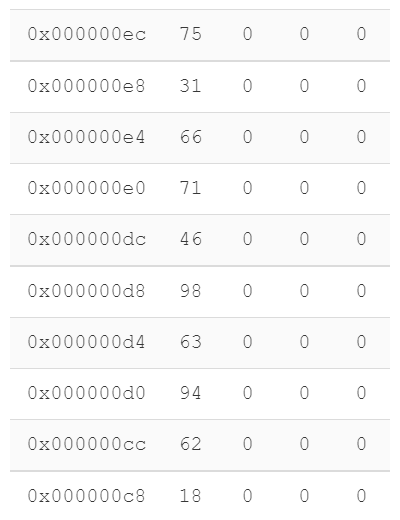
\includegraphics[scale = 1]{../images/Unsorted Array.png}
    \label{img1}
    \caption{Initialized (Unsorted) Array}
\end{figure}
\begin{figure}[H]
    \centering
    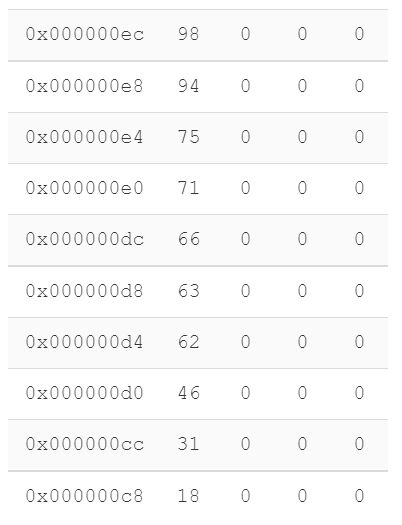
\includegraphics[scale = 1]{../images/Sorted Array.png}
    \label{img2}
    \caption{Sorted Array}
\end{figure}
\subsection*{\Large Modifications in Single Cycle Processor \& Challenges Addressed}
For executing the assembly language code of insertion sort on our lab-made single cycle processor, Following were the required modifications and the way we addressed it.
\begin{itemize}
    \item \textbf{Inclusion of \texttt{blt, bge, bne, beq} Instructions} - As any Sorting Algorithm requires less than, greater than, equal to and not equal to comparisions, therefore there was a need to include these four instructions. To do so, a seperate module named \hyperref[branch_module]{Branch Module} was created. This module, in addition with the Zero Flag also takes a Positve Flag as an input which indicates whether the Operand 1 is greater than Operand 2 or not. The Positive Flag is outputed from \hyperref[alu]{ALU} by simply looking at the most significant bit of the result. So first, we check the branch signal to see if the instruction is a branch instruction. Then, to differentiate between these four branch instructions, we compare their funct3 values along with the zero and the positive flags and the instruction whose specified conditions are matched is set to high and at the same time, the other instructions are set to low. This module also includes a \texttt{to\_branch} output which is high if branch condition is met. So, the AND Gate from our previous design is replaced by this branch module.
    \item \textbf{Addition of Load Word and Store Word Instructions} - The Load Word and Store Word functionality was added in the \hyperref[dmem]{Data Memory}. This required because our insertion sort algorithm is implemented on a word array. So, inorder to differentiate between the Load and Store instructions for Word and Double, the funct3 values of the instructions were checked and based on that the load and store instructions for word and double wereintegrated.
\end{itemize}
\subsection*{\Large Testing and Verification}
For testing purposes, There were 10 outputs added to the \hyperref[dmem]{Data Memory} module. These 10 outpus are for the 10 different indices of the array to be sorted. This is not the art of the Single Cycle Processor, rather they are just hard wired to make the verification easier. Upon Converting the assembly language code into machine code and initlizing it in the \hyperref[imem]{Instruction Memory}, the code was executed and the sorted array can be verified from the waveform shown in \hyperref[img3]{Figure 3}.
\begin{figure}[H]
    \centering
    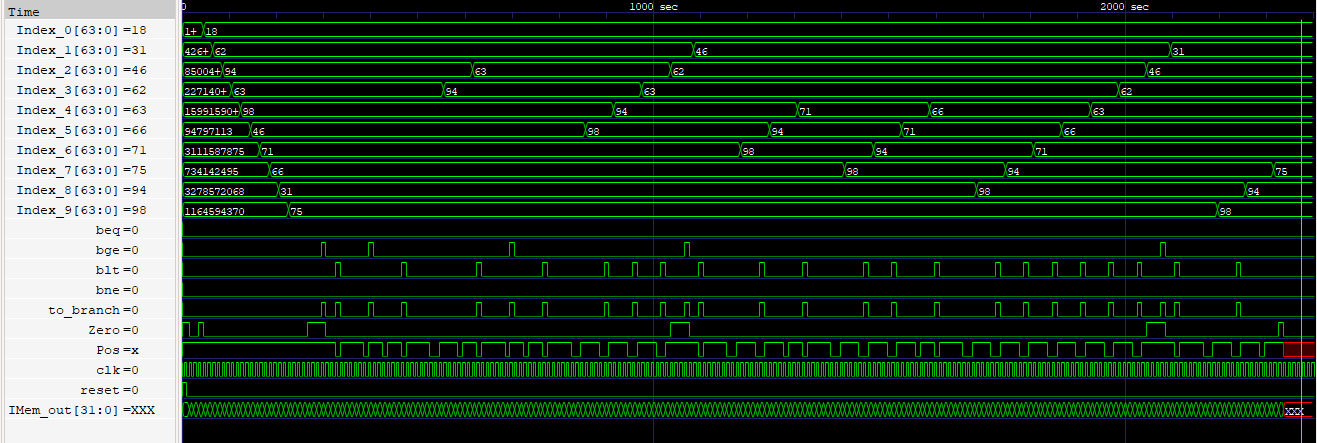
\includegraphics[scale = 0.5]{../images/SCP Wave.png}
    \label{img3}
    \caption{Waveform - Single Cycle Processor}
\end{figure}
\section*{\Huge Task 2 - RISC-V Pipelined Architecture}
\subsection*{\Large Inclusion of 5 Stages and Integration}
\subsection*{\Large Testing Instructions in Isolation}
\section*{\Huge Appendix}
\subsection*{\Large Section 1 - Assembly Language Codes}
\subsubsection*{\large Module 1.1 - Insertion Sort}
\label{ins_sort}
\lstinputlisting[language={[RISC-V]Assembler}]{../Assembly Codes/insertion_sort.asm}
\subsubsection*{\large Module 1.2 - Isolation Tests}
\label{iso}
\lstinputlisting[language={[RISC-V]Assembler}]{../Assembly Codes/isolation_tests.asm}
\subsection*{\Large Section 2 - RISC-V Single Cycle Processor Modules}
\subsubsection*{\large Module 2.1 - Adder}
\lstinputlisting[language = Verilog]{../RISC_V_Single_Cycle/Adder.v}
\subsubsection*{\large Module 2.2 - ALU (64-bit)}
\label{alu}
\lstinputlisting[language = Verilog]{../RISC_V_Single_Cycle/ALU_64_bit.v}
\subsubsection*{\large Module 2.3 - ALU Control}
\lstinputlisting[language = Verilog]{../RISC_V_Single_Cycle/ALU_Control.v}
\subsubsection*{\large Module 2.4 - Branch Module}
\label{branch_module}
\lstinputlisting[language = Verilog]{../RISC_V_Single_Cycle/branch_module.v}
\subsubsection*{\large Module 2.5 - Control Unit}
\lstinputlisting[language = Verilog]{../RISC_V_Single_Cycle/Control_Unit.v}
\subsubsection*{\large Module 2.6 - Data Memory}
\label{dmem}
\lstinputlisting[language = Verilog]{../RISC_V_Single_Cycle/Data_Memory.v}
\subsubsection*{\large Module 2.7 - Immediate Data Generator}
\lstinputlisting[language = Verilog]{../RISC_V_Single_Cycle/imm_data_gen.v}
\subsubsection*{\large Module 2.8 - Instruction Decoder}
\lstinputlisting[language = Verilog]{../RISC_V_Single_Cycle/instruction.v}
\subsubsection*{\large Module 2.9 - Instruction Memory}
\label{imem}
\lstinputlisting[language = Verilog]{../RISC_V_Single_Cycle/Instruction_Memory.v}
\subsubsection*{\large Module 2.10 - MUX (64-bit, 2 by 1)}
\lstinputlisting[language = Verilog]{../RISC_V_Single_Cycle/MUX.v}
\subsubsection*{\large Module 2.11 - Program Counter}
\lstinputlisting[language = Verilog]{../RISC_V_Single_Cycle/Program_Counter.v}
\subsubsection*{\large Module 2.12 - Register File}
\lstinputlisting[language = Verilog]{../RISC_V_Single_Cycle/registerFile.v}
\subsubsection*{\large Module 2.13 - RISC-V Processor (Top Level Module)}
\lstinputlisting[language = Verilog]{../RISC_V_Single_Cycle/RISC_V_Processor.v}
\subsubsection*{\large Module 2.14 - Shift Left}
\lstinputlisting[language = Verilog]{../RISC_V_Single_Cycle/shift_left.v}
\subsubsection*{\large Module 2.15 - Test Bench}
\lstinputlisting[language = Verilog]{../RISC_V_Single_Cycle/tb.v}
\subsection*{\Large Section 3 - RISC-V Pipeline Processor Modules}
\subsubsection*{\large Module 3.1 - Adder}
\lstinputlisting[language = Verilog]{../RISCV_Pipeline/Adder.v}
\subsubsection*{\large Module 3.2 - ALU (64-bit)}
\lstinputlisting[language = Verilog]{../RISCV_Pipeline/ALU_64_bit.v}
\subsubsection*{\large Module 3.3 - ALU Control}
\lstinputlisting[language = Verilog]{../RISCV_Pipeline/ALU_Control.v}
\subsubsection*{\large Module 3.4 - Branch Module}
\lstinputlisting[language = Verilog]{../RISCV_Pipeline/branch_module.v}
\subsubsection*{\large Module 3.5 - Control Unit}
\lstinputlisting[language = Verilog]{../RISCV_Pipeline/Control_Unit.v}
\subsubsection*{\large Module 3.6 - Data Memory}
\lstinputlisting[language = Verilog]{../RISCV_Pipeline/Data_Memory.v}
\subsubsection*{\large Module 3.7 - EX/MEM Stage Register}
\lstinputlisting[language = Verilog]{../RISCV_Pipeline/EX_MEM.v}
\subsubsection*{\large Module 3.8 - Forwarding Unit}
\lstinputlisting[language = Verilog]{../RISCV_Pipeline/forwarding_unit.v}
\subsubsection*{\large Module 3.9 - Hazard Detection Unit}
\lstinputlisting[language = Verilog]{../RISCV_Pipeline/Hazard_Detection.v}
\subsubsection*{\large Module 3.10 - ID/EX Stage Register}
\lstinputlisting[language = Verilog]{../RISCV_Pipeline/ID_EX.v}
\subsubsection*{\large Module 3.11 - IF/ID Stage Register}
\lstinputlisting[language = Verilog]{../RISCV_Pipeline/IF_ID.v}
\subsubsection*{\large Module 3.12 - Immediate Data Generator}
\lstinputlisting[language = Verilog]{../RISCV_Pipeline/imm_data_gen.v}
\subsubsection*{\large Module 3.13 - Instruction Decoder}
\lstinputlisting[language = Verilog]{../RISCV_Pipeline/instruction.v}
\subsubsection*{\large Module 3.14 - Instruction Memory}
\lstinputlisting[language = Verilog]{../RISCV_Pipeline/Instruction_Memory.v}
\subsubsection*{\large Module 3.15 - MEM/WB Stage Register}
\lstinputlisting[language = Verilog]{../RISCV_Pipeline/MEM_WB.v}
\subsubsection*{\large Module 3.16 - MUX (64-bit, 2 by 1)}
\lstinputlisting[language = Verilog]{../RISCV_Pipeline/MUX.v}
\subsubsection*{\large Module 3.17 - MUX (64-bit, 3 by 1)}
\lstinputlisting[language = Verilog]{../RISCV_Pipeline/MUX_3.v}
\subsubsection*{\large Module 3.18 - MUX (ALU Control, 16 by 8)}
\lstinputlisting[language = Verilog]{../RISCV_Pipeline/MUX_Control.v}
\subsubsection*{\large Module 3.19 - Program Counter}
\lstinputlisting[language = Verilog]{../RISCV_Pipeline/Program_Counter.v}
\subsubsection*{\large Module 3.20 - Register File}
\lstinputlisting[language = Verilog]{../RISCV_Pipeline/registerFile.v}
\subsubsection*{\large Module 3.21 - RISC-V Processor (Top Level Module)}
\lstinputlisting[language = Verilog]{../RISCV_Pipeline/RISC_V_Pipeline.v}
\subsubsection*{\large Module 3.22 - Shift Left}
\lstinputlisting[language = Verilog]{../RISCV_Pipeline/shift_left.v}
\subsubsection*{\large Module 3.23 - Test Bench}
\lstinputlisting[language = Verilog]{../RISCV_Pipeline/tb.v}









\end{document}